\chapter{Примеры}

\section{Примеры списков и формул}
\subsection{Примеры списков}

Пример ссылок на источники:
\begin{itemize}
	\item книга про Tex \autocite{book};
	\item как писать формулы \autocite{latexformuls}.
\end{itemize}

Пример нумерованного списка:
\begin{enumerate}
	\item первый пункт;
	\item второй пункт.
\end{enumerate}

\subsection{Примеры формул}

Формула в тексте $\forall x \in X, \quad \exists y \leq \epsilon$.

Формула отдельно \ref{formula:example1}:
\begin{equation}	
	\rho(x,x')=\sqrt[r]{\sum_{i}^{n}(x_i-x_i')^P}
	\label{formula:example1}
\end{equation}

\section{Примеры рисунков и таблиц}

Пример рисунка изображен на рисунке \ref{fig:example1}.
\begin{figure}[h!]
	\centering
	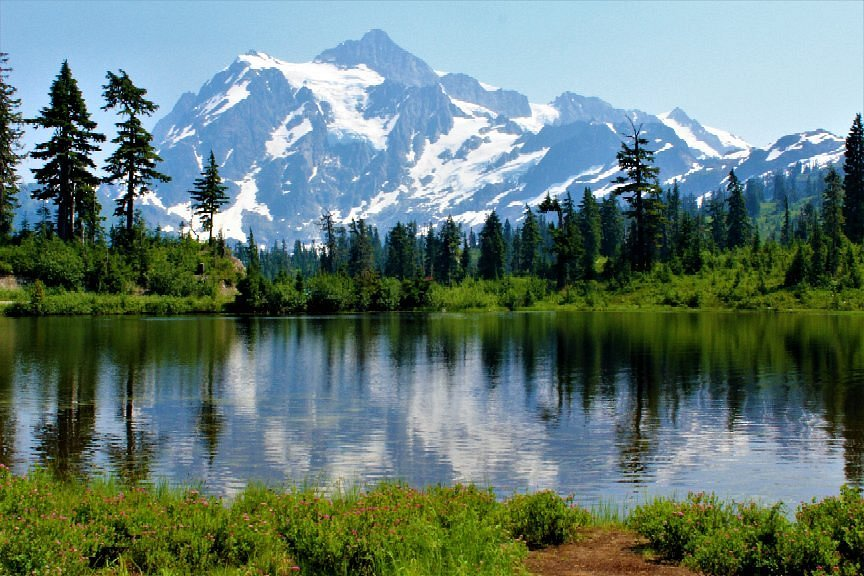
\includegraphics[width=0.7\textwidth]{example1.jpg}
	\caption{Пример рисунка}
	\label{fig:example1}
\end{figure}

Пример таблицы в таблице \ref{table:example1}.

\begin{table}[h!]
\captionstyle{\justifying}
	\caption{Пример таблицы}
		\begin{adjustbox}{width=1\textwidth}
			\small
			\begin{tabular}{|m{3.9cm}|l|m{3cm}|}
				\hline
				\textbf{Колонка 1} & \textbf{Колонка 2} & \textbf{Колонка 3} \\ \hline
				поле 1.1 & поле 2.1 & поле 3.1 \\ \hline
				поле 1.2 & поле 2.2 & поле 3.2 \\ \hline
				поле 1.3 & поле 2.3 & поле 3.3 \\ \hline
			\end{tabular}
		\end{adjustbox}	
	\label{table:example1}
\end{table}